\documentclass{article}
\usepackage[utf8]{inputenc}

\usepackage{amsmath}
\usepackage{graphicx}
\usepackage{indentfirst}

%--------Margin of the page------------%
\usepackage[margin=1in]{geometry}

%--------Code Snipplet Setting------------%
\usepackage{listings}
\usepackage{xcolor}

\definecolor{codegreen}{rgb}{0,0.6,0}
\definecolor{codegray}{rgb}{0.5,0.5,0.5}
\definecolor{codepurple}{rgb}{0.58,0,0.82}
\definecolor{backcolour}{rgb}{0.95,0.95,0.92}

\lstdefinestyle{mystyle}{
    backgroundcolor=\color{backcolour},   
    commentstyle=\color{codegreen},
    keywordstyle=\color{magenta},
    numberstyle=\tiny\color{codegray},
    stringstyle=\color{codepurple},
    basicstyle=\ttfamily\footnotesize,
    breakatwhitespace=false,         
    breaklines=true,                 
    captionpos=b,                    
    keepspaces=true,                 
    numbers=left,                    
    numbersep=5pt,                  
    showspaces=false,                
    showstringspaces=false,
    showtabs=false,                  
    tabsize=2
}

\lstset{style=mystyle}
%--------Code Snipplet Setting------------%

\begin{document}

\section*{Newton line search algorithm}

Finding the minimizer(s) of $f$ is resemble to finding the root(s) of $f'$. From 
$$f(x) = 10(x-1)^4 - 4\sin(3x)$$

Then, a derivative of this function w.r.t. $x$ is given here:
$$f'(x) = 40(x-1)^3 - 12\cos(3x)$$

Let $g(x) = f'(x)$. Now, we will use the Newton-Raphson method to find the root of $g(x)$. Then, the formula will be:
\begin{align*}
    x_{k+1} &= x_k + g(x_k)/g'(x_k) \\
        &= x_k + \frac{40(x-1)^3 - 12\cos(3x)}{120(x-1)^2 + 36\sin(3x)}
\end{align*}

MATLAB can be very useful for this. The code used to solve this problem is adapted from the last homework. The \lstinline{FunctionName.m} is modified to

\lstinputlisting[language=Matlab]{FunctionName.m}

The \lstinline{newton.m}, however, do not need to be modified at all.

\lstinputlisting[language=Matlab]{newton_1var.m}

The result is printed by this script.

\lstinputlisting[language=Matlab]{script_test.m}

And the printed result is written below:

\lstinputlisting[]{result.txt}

So, the value of a minimizer of $f$ is 0.5969431100.

To determine whether $f$ has only one minimizer, let's analyze from the function derivative: 
$$f'(x) = 40(x-1)^3 - 12\cos(3x)$$

Plot the graph of $40(x-1)^3$ and $12\cos(3x)$ in the same area.

\begin{figure}[h]
    \centering
    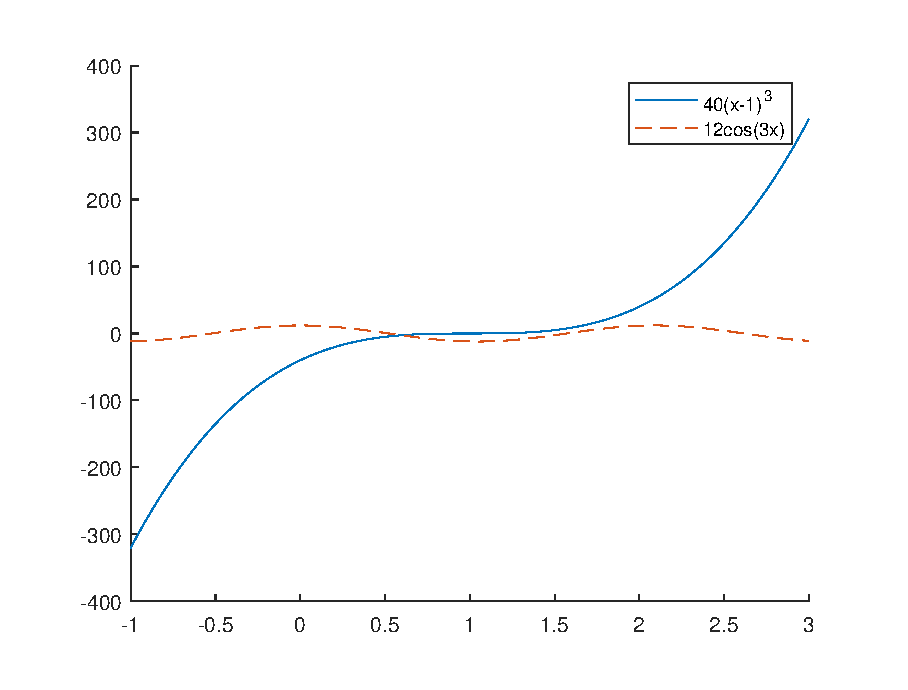
\includegraphics[width = 0.7\textwidth]{plot.eps}
    \caption{The graph of $40(x-1)^3$ and $12\cos(3x)$.}
\end{figure}

From the graph, for $x < 0.597$, $40(x-1)^3 < 12\cos(3x)$ so $f'(x)$ is always negative. For $x \geq 0.597$, $40(x-1)^3 \geq 12\cos(3x)$ so $f'(x)$ is always positive. Therefore $f'(x)$ has only one root, then $f(x)$ has only one minimizer.

\end{document}